\lab{Pseudorandom Number Generators}{Pseudorandom Number Generators}
\label{lab:PRNG}

\objective{Learn about the strengths and weaknesses of a few pseudorandom number generators}

\section*{Random Numbers}
Lotteries, most board games, and statistics need random numbers.
In real life, we roll dice, take balls out of a bag, or spin a wheel.
Computers are, by nature, deterministic, meaning that they do exactly what they are told.
Because of this, random number generation on a computer can be difficult.
We can have a device measure a random process and use the data to generate random numbers, 
but such sampling is often too slow and too expensive for practical use.
Pseudorandom number generators (PRNGs) are a common solution to this problem.
The numbers are not truly random, but they are based on a complex formula that makes them look ``random."
For convenient use, these generators must also run quickly.
The goal is to have something that is fast and looks random.

There are many different algorithms for developing pseudorandom numbers.
Robert R. Coveyou titled an article ``The generation of random numbers is too important to be left to chance."
There has been much study about different PRNGs.
This lab will cover Linear Congruential Generators.

\section*{Linear Congruential Generators}
Linear Congruential Generators (LCGs) are one of the oldest ways of generating random numbers.
The generator is defined by the recurrence relation:
$X_{n+1}=(a*X_n + c)$ mod $m$ where

\begin{itemize}
\item $X$ is a sequence of pseudorandom values
\item $m$ is the modulus, with $m>0$
\item $a$ is the multiplier, with $0<a<m$
\item $c$ is the increment, with $0\leq c<m$
\item $X_0$ is the seed, with $0\leq X_0 <m$
\end{itemize}

The $a$, $m$, $c$, and $X_n$ are integer constants.

\begin{problem}\label{LCG1}
Write an LCG that produces an array of pseudorandom numbers between $0.0$ and $1.0$.
Define your LCG to take the size of the array as an argument, and let $a$, $c$, $m$, and $seed$ be optional arguments.
For the purpose of this example, let $a=1103515245$, $c=12345$, $m=2^{31}-1$, and $seed=4329$ be the default values.
\end{problem}

\begin{problem}
Write an LCG that produces an array of pseudorandom numbers of integers between two input arguments.
Do it by calling your algorithm from problem \ref{LCG1} and multiplying it by the values and casting the array as an integer using \li{.astype()}.
Let the arguments be the size of the array and the two integers.
Let $a$, $c$, $m$, and $seed$ continue to be optional arguments.
\end{problem}

This algorithm is used as the default random number generator in Java and C++, and is still used in a wide variety of situations.
The length over which your random number generator repeats is called the period.
The period is at most $m$, but it may be shorter based on the values of $a$ and $c$.

\begin{figure}

\includegraphics[width=.4\textwidth]{PRNG1.png}
\caption{
The bitmap with $a=3$, $c=2$, $m=2^{16}$.
There is a clear pattern in the random numbers.}
\end{figure}

One easy way to ``see" if your generator is random is to look at a bitmap of the output.
In python, you will need to import matplotlib and use \li{.imshow()} to see a bitmap of the array produced by your LCG.
Resize your output to be $512 \times 512$ (you will need $512^2$ random numbers in your array).



\begin{problem}
For what values of $a$, $c$, and $m$ does your LCG have a visible pattern?

Look at the bitmap for the output of \li{np.random.rand(512, 512)}.
Can you see any patterns?
\end{problem}


 
\begin{comment}
According to the Hull-Dobell Theorem (TO DO: find a source), a LCG will have a full period if and only if, 
1. $c$ and $m$ are relatively prime,
2. $a-1$ is divisible by all prime factors of $m$,
3. $a-1$ is a multiple of 4 if $m$ is a multiple of 4

\begin{problem}
Test values of $a$,$c$, and $m$ that fit these requirements. 
\end{problem}
\end{comment}




\begin{comment}
\section*{Mersenne Twister}
(TO DO: decide how much of  this we want to keep) All numbers can be represented in bits as a base two number.
Computers are optimized to work with numbers in that manner.
The operators XOR, OR, and AND work on the bit representation of two numbers.

AND - if both numbers have a 1 in the ith place then the ith place is 1.
Otherwise the ith place is 0.

OR - if one or both numbers have a 1 in the ith place then the ith place is 1.
Otherwise the ith place is 0.

XOR - if only one of the two numbers has a 1 in the ith place then the ith place is 1.
If both or neither of the numbers has a 1 in the ith place, the ith place is 0.

In addition you can shift the bitwise number over a number of values.
For example, shifting 10100 to the right by one yields 1010 and shifting it to the left by one yields 101000.
This is really just division and multiplication by 2.
This can be done by $\ll$ and $\gg$ in python. 


The Mersenne twister PRNG does a series of bitwise operations to generate random numbers.
The Random class in python uses the Mersenne twister algorithm. 

\begin{problem}
Look at the bitmap for the of output of \li{np.random.rand(512, 512)}.
Can you see any patterns?
\end{problem}

\section*{Randomness Tests}
Many statistical tests have been devised to measure the quality of a random number generator.
One of these tests is the overlapping permutations test.
This test involves taking an arbitrarily large collection of sequences of five consecutive random numbers from the generator and finding the probability that one of the 120 possible permutated orderings occurs.
In a good PRNG, the 120 orderings should occur with equal probability.

To simplify this process, instead of considering a specific sequence of five consecutive random numbers, consider the argsort of this sequence.
For example: instead of considering how often the sequence $[103, 75, 4, 57, 9]$, or any permutation thereof, shows up, consider argsort([103, 75, 4, 57, 9])=[2, 4, 3, 1, 0]$ (Remember, argsort gives index of increasing values in the array).
In this sense, we can now look at the frequency with which the permutations of 0, 1, 2, 3, and 4 show up under argsort.

It is convenient to use the $plt.bar()$ command under $matplotlib$ to generate a Histogram of the number of times each permutation shows up in the collection of sequences.

\begin{problem}
Use the overlapping permutations test to see how random python's random number generator is compared to the LCG you wrote in problem 1.
Create a bar graph with 120 bins, one for each ordering, to view graphically the difference. (Hint: Consider using a dictionary to store all possible orderings)
\end{problem}

\end{comment}

\section*{Blackjack}
\begin{figure}
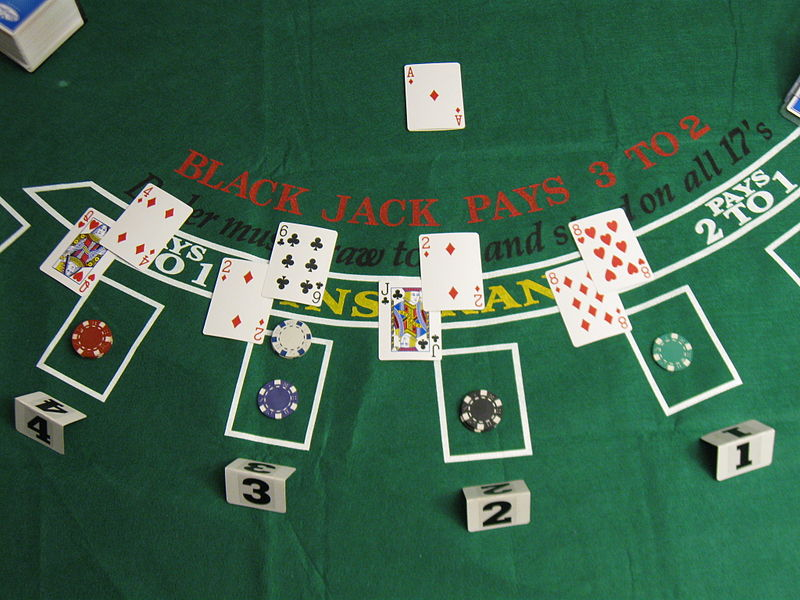
\includegraphics[width=\textwidth]{Blackjack_game_1.jpg}
\caption{Initial Round of a Blackjack game.}
\end{figure}

Blackjack is a card game that involves the use of randomness.
The game is simple.
The dealer deals the player and himself each two cards.
He flips over his first card so that the player can see it.
The player has to choose to take another card ("hit") or not ("stand").
If the player hits he gets another card and again has the choice to hit or stand.

The goal is to get your hand to be at or as close to 21 without going over.
Face cards are worth 10 points.
Aces can count either as 11 or 1.
The value of all other cards are equal to the number on the card.

Once the player has decided to stand the dealer flips over his second card and deals himself cards until his hand value is 17 or greater. 

If the player's value goes above 21 he automatically loses.
If his value is 21 or below and the dealer has above 21 then the player wins.
If they both have 21 or under then the player with the hand of highest value wins.
If both hands have the same value, the game is a tie.

\section*{Shuffling Algorithms}
One use of PRNGs is to shuffle cards.
The main goal of these algorithms is to make the card order be random--so that no single player has an advantage based on order.
Often, as strange as it may seem, online gambling sites will post their shuffling algorithms online; the only things they do not post are their seed values.
Often the time in milliseconds from midnight is used as the seed value.

John von Neumann said, ``Anyone who considers arithmetical methods of producing random digits is, of course, in a state of sin."
As seen in the first part of this lab, weak PRNGs are periodic and are predictable once a few outputs are known.
Now we will have you break Blackjack based on a weak PRNG.

\section*{Cracking Blackjack}
For these next problems you will need three files that are provided with this lab: BlackHard.py, BlackEasy.py, and bjCommon.py.
BlackHard.py and BlackEasy.py are programs that run games of Blackjack that use an LCG to shuffle the cards.
They generate 52 random numbers and then use the natural ordering of those numbers as the ordering of the cards.
The parameters for BlackEasy.py are $a=2521$, $c=13$, $m=2^{16}$.
For BlackHard.py they are $a=25214903917$, $c=11$, $m=2^{48}$.

\begin{warn}
Both BlackEasy.py and BlackHard.py use functions that are incompatible with ipython.
To run them, use \li{python <<filename>><<numberofgames>>} in the command line.
\end{warn}

BlackEasy.py uses a seed randomly generated between 0 and 10000000.
The seed for BlackHard.py is based on the time, using \li{ (int)(time.time())}, which is the number of seconds from the start of the epoch cast as an integer.
(This can be found in the time package).
Both programs will make a list of length \li{<<numberofgames>>}, where each element in the list is a shuffling of the deck.
During each round, the program will choose the next deck in your list generated.
Cards are popped off the deck one at a time: first one to the player, second one to the dealer, third one to the player, and one last one to the dealer. 

Initially three cards are visible (the last of the dealer's is face down) so our algorithms will deal with these first three cards, and the ordering (player, dealer, player) will be very important. 
After the first four cards are down the next cards are popped off in the order that they appear. 

bjCommon.py contains several functions to help you with the game's mechanics.
Cards have a string representation ( '6diamond' for 6 of diamonds, 'Kclub' for king of clubs, 'Aheart' for ace of hearts, and so on) and a number representation that determines their natural ordering. 
bjCommon.py has functions for generating the list of cards and converting arrays to and from the string and integer representation of cards. 
Particularly useful is the function \li{shuffle}, which when given the number of games, $g$, the LCG parameters, and a seed value, returns the first $g$ decks (or games) in integer representation as $g$ arrays of 52 integers.

Your goal will be to do a sweep of seed values and cross check the decks produced by \li{shuffle} against the first three cards from several games, then be able to determine the order of cards for future rounds.


\begin{problem}\label{sweeps}

Create a function, \li{getSweepsEasy(games,n)}, which has as its parameters the number of games you selected to play in BlackEasy.py and a seed value.
The function needs to return an array of size $n\times games \times 52$, representing all possible seed values 0 through $n$ in the first dimension, the different shufflings that occur based on the number of games played in the second dimension, and the ordering of the 52 cards for each shuffle in the third dimension.
(Be sure to look at \li{bjCommon.shuffle} to help get the needed results)

What seed value $n$ would you use to make sure to cover all possible shufflings?
(Look at the parameters of the LCG in BlackEasy.py]).

\end{problem}

From problem \ref{sweeps}, using the right value for $n$ will get you the list of all possible initial shuffles, as well as the appropriate number of future hands depending on the games parameter.
Once we have the possible shufflings, we want a convenient way to match the output from BlackEasy.py with the output from problem \ref{sweeps}.
The function \li{bjCommon.findSeedMatch} provides us the means of comparing these two outputs.
It takes as parameters sweeps, game, and cardNames3; sweeps is the output from problem \ref{sweeps} (an $n \times games \times 52$ array), game is the round number, and cardNames3 is a 3-tuple of the names of the first three cards dealt out (using the naming notation mentioned above).

\begin{problem}

Create a function \li{crackBlackJack(sweeps, cardTuples)} to crack the shuffling algorithm of BlackEasy.py.
The parameter sweeps represents the output from problem \ref{sweeps}.
The parameter cardTuples is a list of 3-tuples from the 1st, 2nd, etc. rounds played.
It should return a subset of shuffles from sweeps whose shuffles match in each round to each 3-tuple in cardTuples.

Be sure to make use of \li{bjCommon.findSeedMatch} and \li{bjCommon.convertToName} to see the names associated to the orderings of cards.

\end{problem}

Keep in mind the key difference between BlackEasy.py and BlackHard.py is the seed that is used and the value $m$ which the shuffling algorithm mods out by for each shuffle.
BlackEasy.py has a small selection of seeds to choose from, while BlackHard.py uses a seed based on time, which can get pretty big.
While in BlackEasy.py you could easily find all possible seed values and the corresponding shuffles, in BlackHard.py you will need to know the approximate time you initiated the game.
This can be done using the \li{time.time()} function shortly after initializing BlackHard.py in python.

\begin{problem}

Create a function, \li{getSweepsHard(games, time, approx=120)}, which returns all possible shuffles for a range of seed values.
The parameter games is how many rounds you want to play (corresponding to different shuffles of a given seed value).
The time parameter is the approximate time you started the round of BlackHard.py.
The approx parameter will give a range of seed values (120 seconds before and after the approximate time you initiated the game).
It should return a $(2*approx) \times games \times 52$ array of possible shuffles, similar to problem \ref{sweeps}.

You should be able to run \li{crackBlackJack} using this output to help determine future rounds of BlackHard.py.

\end{problem}
